\documentclass[../main.tex]{subfiles}

\begin{document}
\chapter{Das Riemannsche Integral}
Das Riemannsche Integral wurde
vom Schüler Bernhard Riemann (1826--1866)
von Gauss eingeführt.

Sei $f \colon \mathbb{R} \to \mathbb{R}$ differenzierbar
mit $f' = 0$ (die Nullfunktion).
Dann ist $f$ konstant (was wir bereits mithilfe des
Mittelwertsatz gezeigt haben). Daraus können wir
folgendes schliessen.
Seien $f, g \colon \mathbb{R} \to \mathbb{R}$ 
differenzierbare
Funktionen mit
$f' = g'$, das heisst, für alle $x \in \mathbb{R}$
gilt $f'(x) = g'(x)$.
Dann ist $f - g$ konstant.
Wir folgern, dass die Funktion $f \colon \mathbb{R} \to \mathbb{R}$ 
durch ihre Ableitung $f' \colon \mathbb{R} \to \mathbb{R}$ 
und einen Wert $f(0)$ determiniert ist.

\begin{question}
  Wie bestimmen wir $f$ aus $f'$ 
  und $f(0)$?
\end{question}

\begin{specialcase}
  Sei $f$ affin. Dann gilt für alle
  $x \in \mathbb{R}$, dass
  \[
    f(x) = f(0) + x \cdot f'(0).
  \]
  Dies gilt im Allgemeinen nicht: wir verwenden
  hier, dass $f$ affin ist.
  Aber immerhin ist für kleine $|h|$
  der Ausdruck $f(x) + h \cdot f'(x)$ eine
  gute Approximation von $f(x + h)$.
\end{specialcase}

Dies führt zu der Überlegung, dass für beliebige
Funktionen der Ausdruck
\[
  f(x) = f(0) + (f(x/N) - f(0))
  + (f(2x/N) - f(x/N)) + \cdot
  + (f(x) - f((N-1)x/N))
\]
zu einer Approximation von $f$ aus
$f'$ führen könnte. Für grosse $N$ 
sollte nämlich
\[
  f(x) - f(0) \approx \sum_{k = 0}^{N - 1} 
  \frac{x}{N} \cdot f'(k \cdot x / N)
\]
eine gute Approximation sein, wobei
hier das Symbol $\approx$ für ein
saloppes ``ungefähr'' steht.
Im Grenzübergang erhalten wir das
Integral
\[
  \int_{0}^{x} f'(t) \, dt =
  \lim_{N \to \infty} \sum_{k = 0}^{N - 1} \frac{x}{N}
  f'(k \cdot x/N).
\]
Nun definieren wir dieses Integral formal.

\section{Die Definition des Riemannschen Integrals}\label{sec:riemann-definition}
\begin{definition}
  Seien $a,b \in \mathbb{R}$
  mit $a < b$. Eine \emph{Partition} des Intervalls
  $[a, b]$ ist eine Unterteilung in
  endlich viele Teilintervalle der
  Form
  $I_k = [x_k, x_{k  + 1}]$ mit
  \[
    a = x_0 < x_1 < \cdots < x_n = b.
  \]
  Wir notieren diese Partition als
  $P = [x_0, x_1, \dots, x_n]$.
\end{definition}

Sei nun $f \colon [a, b] \to \mathbb{R}$ von oben und
unten beschränkt und $P$ eine Partition von $[a, b]$.
Definiere die korrespondierende \emph{Obersumme} durch
\[
  \overline S_P(f)
  = \sum_{k = 0}^{n - 1} (x_{k + 1} - x_k)
  \cdot \sup \left\{f(x) \mid x \in I_k \right\}
\]
und die korrespondierende \emph{Untersumme} durch
\[
  \underline S_P(f)
  = \sum_{k = 0}^{n - 1} (x_{k + 1} - x_k)
  \cdot \inf \left\{f(x) \mid x \in I_k \right\},
\]
siehe Abbildung~\ref{fig:riemann}.

\begin{figure}[htb] 
  \centering
  \begin{minipage}{0.50\textwidth}
    \centering

    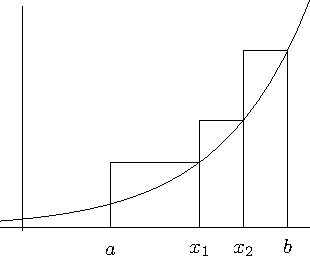
\includegraphics{images/sum-upper}
  \end{minipage}%
  \begin{minipage}{0.50\textwidth}
    \centering

    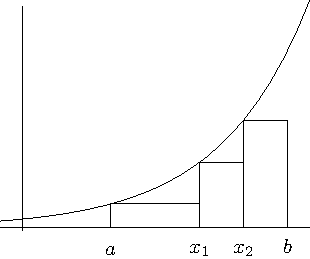
\includegraphics{images/sum-lower}
  \end{minipage}%
  \caption{Obersumme und Untersumme}%
  \label{fig:riemann}
\end{figure}

\begin{lemma*}
  Seien $P_1$ und $P_2$ Partitionen
  von $[a, b]$. Dann gilt
  $\underline S_{P_1} \leq \overline S_{P_2}$.
  In anderen Worten sind alle Untersummen
  kleiner als alle Obersummen.
\end{lemma*}

\begin{proof}
  Schreibe
  $P_1 = [x_0, x_1, \dots, x_n]$ 
  und
  $P_2 = [y_0, y_1, \dots, y_m]$.
  Wähle eine Partition $Q$ von
  $[a,b]$, welche alle $x_i$ und
  $y_j$ enthält, eine sogenannte
  \emph{gemeinsame Verfeinerung}
  von $P_1$ und $P_2$.
  Dann gilt
  \[
    \underline S_{P_1} \leq \underline S_Q
    \leq \overline S_Q
    \leq \overline S_{P_2}.
  \]
  Dass die Untersummen beim Verfeinern
  grösser und die Obersummen kleiner
  werden, ist eine kleine Übung.
\end{proof}

\begin{definition}
  Eine beschränkte Funktion
  $f \colon [a, b] \to \mathbb{R}$ heisst
  \emph{Riemann-integrierbar}, falls
  \[
    \sup_{P} \underline S_P(f) = \inf_{Q} \overline S_Q(f)
  \]
  gilt,
  wobei $P$ und $Q$ alle Partitionen von
  $[a, b]$ durchlaufen.
  Diese Zahl heisst dann \emph{Riemann-Integral}
  von $f$ über $[a,b]$ und wird
  mit
  \[
    \int_{a}^{b} f(x) \, dx
  \]
  notiert.
\end{definition}

\begin{examples}
  \leavevmode
  \begin{enumerate}[(1)]
    \item Betrachte die Funktion
      \begin{align*}
        f \colon [0, 1] & \to \mathbb{R} \\
        x & \mapsto 
        \begin{cases}
          1 & \text{falls $x \in \mathbb{Q}$},\\
          0 & \text{falls $x \in \mathbb{R} \setminus \mathbb{Q}$}.
        \end{cases}
      \end{align*}
      Für alle Partitionen $P$ von $[0, 1]$ gilt
      \[
        \overline S_P(f) = 1
      \]
      und
      \[
        \underline S_P(f) = 0.
      \]
      Also ist $f$ nicht Riemann-integrierbar.
    \item Betrachte die Funktion
      \begin{align*}
        f \colon [-1, 1] & \to \mathbb{R} \\
        x & \mapsto 
        \begin{cases}
          0 & \text{falls $x \leq 0$},\\
          1 & \text{falls $x > 0$}.
        \end{cases}
      \end{align*}
      Betrachte die Partition
      $P = [-1, 0, 1/N, 1]$ für festes $N \in \mathbb{N}$.
      Es gilt
      \[
        \overline S_P(f) = 1
      \]
      und
      \[
        \underline S_P(f) = 1 - 1/N.
      \] 
      Somit folgt $\overline S_P - \underline S_P = 1/N$,
      also ist $f$ Riemann-integrierbar und es gilt
      \[
        \int_{-1}^{1} f(x) \, dx = 1.
      \]
  \end{enumerate}
\end{examples}

\begin{theorem}\label{thm:continuous-integrable}
  Sei $f \colon [a, b] \to \mathbb{R}$ stetig. Dann ist $f$ 
  Riemann-integrierbar.
\end{theorem}

\begin{proof}
  Da $[a, b]$ kompakt ist, impliziert die Stetigkeit von $f$ sogar
  \emph{gleichmässige Stetigkeit} auf $[0, 1]$:
  Für alle $\varepsilon > 0$ existiert $\delta > 0$ so, dass
  für alle $p, q \in [a, b]$ mit $|q - p| \leq \delta$ gilt, dass
  $|f(q) - f(p)| \leq \varepsilon$.
  Wähle $N \in \mathbb{N}$ mit
  \[
    \frac{b-a}{N} \leq \delta.
  \]
  Betrachte die Partition
   \[
    P = \left[ a, a + \frac{b - a}{N}, a + 2 \frac{b-a}{N}, \dots,
    b\right].
  \]
  Für diese gilt
  \begin{align*}
    \overline S_P(f) - \underline S_P(f)
    &\leq \sum_{k=0}^{N-1} \frac{b-a}{N}\cdot \varepsilon  \\
    & N \frac{b-a}{\varepsilon} \\
    &= \varepsilon \cdot (b-a).
  \end{align*}
  Wir folgern, dass die Differenz $\overline S_P(f) - \underline S_P(f)$ 
  beliebig kleine Werte annehmen kann. Insbesondere gilt,
  dass
  \[
    \lim_{N \to \infty} \overline S_P(f) - \underline S_P(f) = 0.
  \]
  Folglich ist $f$ Riemann-integrierbar.
\end{proof}

\begin{example}
  Betrachte die Funktion
  \begin{align*}
    f \colon [0, 1] & \to \mathbb{R} \\
    x & \mapsto x^n
  \end{align*}
  für $n \in \mathbb{N}$ beliebig. Betrachte die
  Partition
  \[
    P = [0, 1/N, 2/N, \dots, 1].
  \]
  Es gilt:
  \[
    \overline S_P(f) = \frac{1}{N} \cdot \left( {\left( \frac{1}{N}  \right)}^n
    + \cdots + {\left( \frac{N}{N}  \right)}^n \right)
  \]
  und
  \[
    \underline S_P(f) = \frac{1}{N} \cdot \left( 0 +{\left( \frac{1}{N}  \right)}^n 
    + \cdots + {\left( \frac{N-1}{N}  \right)}^n\right).
  \]
  Also folgt
  \[
    \lim_{N \to \infty} \overline S_P(f) - \underline S_P(f) = 
    \lim_{N \to \infty}\frac{1}{N} = 0,
  \]
  was wir auch aus Theorem~\ref{thm:continuous-integrable} schliessen konnten.
  Wir wissen aber immer noch nicht, was das Integral
  \[
    I = \int_{0}^{1} x^n \, dx
  \]
  für einen Wert hat.
\end{example}

\begin{geometric}
  Das Integral
  \[
    \int_{a}^{b} f(x) \, dx
  \]
  ist der Flächeninhalt zwischen der $x$-Achse und dessen
  Funktionsgraph zwischen $a$ und $b$ mit Gewichtung
  wie in Abbildung~\ref{fig:riemann-integral}.
  Wir werden dies als Definition des Wortes
  \textit{Flächeninhalt} auffassen.
\end{geometric}

\begin{figure}[htb]
  \centering
  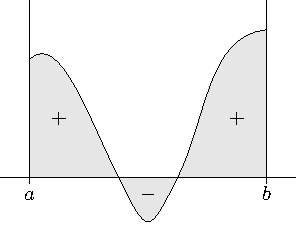
\includegraphics{images/riemann-integral}
  \caption{Die Vorzeichen der Flächen}%
  \label{fig:riemann-integral}
\end{figure}

\begin{remark}
  Stetigkeit in allen Punkten von $[a, b]$ ist
  nicht notwendig: Es gibt unstetige Funktionen,
  die Riemann-integrierbar sind.
\end{remark}

\begin{examples}
  \leavevmode
  \begin{enumerate}[(i)]
    \item Die Funktion
      \begin{align*}
        f \colon [-1, 1] & \to \mathbb{R} \\
        x & \mapsto 
        \begin{cases}
          0 & x \leq 0,\\
          1 & x > 0.
        \end{cases}
      \end{align*}
      ist nicht stetig, aber dennoch Riemann-integrierbar.
    \item Die Funktion
      \begin{align*}
        f \colon [0, 1] & \to \mathbb{R} \\
        x & \mapsto 
        \begin{cases}
          0 & x = 0 \\
          1/x & x > 0
        \end{cases}
      \end{align*}
      ist unbeschränkt und deshalb nicht Riemann-integrierbar.
      Für alle Partitionen $P$ von $[0, 1]$ gilt
      $
      \overline S_P(f) = + \infty$.
      Dieses Phänomen ist der Grund dafür, dass
      wir Beschränktheit von $f$ fordern.
  \end{enumerate}
\end{examples}

\subsection*{Integrabilitätskriterium von Lebesgue}
Henri Lebesgue (1875--1941) war ein Französischer Mathematiker.
Sein Kriterium für Integrabilität charakterisiert die
Riemann-integrierbaren Funktionen, im Gegensatz zu
Theorem~\ref{thm:continuous-integrable}, was nur eine
hinreichende Bedingung darstellt.

\begin{definition}
  Eine Teilmenge $\Delta \subset \mathbb{R}$ 
  heisst \emph{Lebesgue Nullmenge},
  falls für alle $\varepsilon > 0$ abzählbar viele
  offene Intervalle
  \[
    I_k = (a_k, b_k)
  \]
  mit $k \in \mathbb{N}$
  existieren, so dass 
  \[
    \Delta \subset \bigcup_{k=0}^{\infty} I_k
  \]
  und
  \[
    \sum_{k=0}^{\infty} b_k - a_k \leq \varepsilon.
  \]
\end{definition}

\begin{example}
  Sei $\Delta = \mathbb{Q} \subset \mathbb{R}$.
  Sei $\varepsilon > 0$ vorgegeben.
  Wähle eine Bijektion $q \colon\mathbb{N} \to \mathbb{Q}$ 
  und schreibe $q_k = q(k)$ für $k \in \mathbb{N}$.
  Setze
  \[
    a_k = q_k - \frac{\varepsilon}{4} \cdot \frac{1}{2^k}
  \]
  und
  \[
    b_k = q_k + \frac{\varepsilon}{4} \cdot \frac{1}{2^k}.
  \]
  Es gilt $q_k \in (a_k, b_k)$ und  
  \[
    b_k - a_k = \frac{\varepsilon}{2^{k+1}}.
  \]
  Es folgt, dass
  \[
    \sum_{k=0}^{\infty} b_k - a_k = \varepsilon \cdot
    \sum_{k=0}^{\infty} \frac{1}{2^{k+1}} = \varepsilon.
  \]
  Wir haben also $\mathbb{Q}$ abgedeckt mit Intervallen,
  deren Gesamtlänge kleiner als $\varepsilon$ ist.
  Also ist $\mathbb{Q}$ (und, mit dem selben Beweis,
  jede abzählbare Teilmenge von $\mathbb{R}$)
  eine Lebesgue Nullmenge.
\end{example}

\begin{theorem}[Lebesgue 1901]
  Sei $f \colon [a, b] \to \mathbb{R}$ eine Funktion.
  Dann sind folgende Aussagen äquivalent.
  \begin{enumerate}[\normalfont(i)]
    \item $f$ ist  Riemann-integrierbar,
    \item $f$ ist beschränkt und die Menge
      $\Delta$ der Unstetigkeitsstellen von $f$ ist
      eine Lebesgue Nullmenge.
  \end{enumerate}
\end{theorem}

\begin{proof}
  Siehe zum Beispiel Abschnitt 84 in~\cite{heuser}.
\end{proof}

In anderen Vorlesungen, zum Beispiel Analysis 3, wird
der Begriff der Lebesgue-Integrabilität diskutiert.
Mit dem Lebesgue-Integral sind sogar noch mehr Funktionen
integrierbar.

\begin{example}
  Die Funktion
  \begin{align*}
    f \colon [0, 1] & \to \mathbb{R} \\
    x & \mapsto 
    \begin{cases}
      1/q & \text{falls $x = p/q \in \mathbb{Q}$ gekürzt ist},\\
      0 & \text{falls $x \in \mathbb{R} \setminus Q$}
    \end{cases}
  \end{align*}
  ist beschränkt
  und auf $\mathbb{R} \setminus \mathbb{Q}$ stetig,
  also Riemann-integrierbar. In den Übungen wird das
  ``zu Fuss'' mit der Definition des Riemann-Integrals
  gezeigt.
\end{example}

\subsection*{Elementare Eigenschaften des Riemann-Integrals}
\begin{notation}
  Die Menge $R[a, b]$ ist definiert als
  die Menge aller Riemann-integrierbaren Funktionen
  $f \colon [a, b] \to \mathbb{R}$.
\end{notation}

Wir stellen fest:
\begin{enumerate}[(i)]
  \item $R[a, b]$ ist ein reeller Vektorraum.
  \item die Abbildung
    \begin{align*}
      \int \colon R[a,b] & \to \mathbb{R} \\
      f & \mapsto \int_{a}^{b} f(x) \, dx
    \end{align*}
    ist linear.
\end{enumerate}
Konkret heisst das folgendes.
\begin{enumerate}[(i)]
  \item Seien $f, g \colon [a, b] \to \mathbb{R}$
    Riemann-integrierbar und $\lambda \in \mathbb{R}$.
    Dann ist $f + \lambda g \colon [a, b] \to \mathbb{R}$ 
    auch Riemann-integrierbar.
  \item Die Gleichung
    \[
      \int_{a}^{b} f(x) + \lambda g(x) \, dx
      = \int_{a}^{b} f(x) \, dx
      + \lambda \cdot \int_{a}^{b} g(x) \, dx
    \]
    ist für alle Riemann-integrierbaren 
    $f, g \colon [a, b] \to \mathbb{R}$ 
    erfüllt.
\end{enumerate}

\begin{remark}
  Der Vektorraum $R[a,b]$ ist unendlichdimensional, da die
  Funktionen 
  \[
   x \mapsto x^k 
  \]
  linear unabhängig sind.
\end{remark}

An dieser Stelle halten wir ausserdem fest, dass
für alle $c \in [a, b]$ und alle Riemann-integrierbaren
$f \colon [a, b] \to \mathbb{R}$ gilt, dass
\[
  \int_{a}^{b} f(x) \, dx = \int_{a}^{c} f(x) \, dx
  + \int_{c}^{b} f(x) \, dx.
\]

\section{Der Hauptsatz der Differential- und Integralrechnung}
\begin{definition}
  Sei $f \colon [a, b] \to \mathbb{R}$ eine Funktion.
  Eine differenzierbare
  Funktion $F \colon [a, b] \to \mathbb{R}$ ist
  eine \emph{Stammfunktion} von $f$, falls für
  alle $x \in [a, b]$ gilt, dass $F'(x) = f(x)$.
  Hier einigen wir uns auf die Konvention,
  dass Differenzierbarkeit im Punkt $a$ bedeutet, dass
  der Grenzwert
  \[
    F'(a) 
    = \lim_{h \to 0} \frac{F(a + |h|) - F(a)}{|h|} \in \mathbb{R}
  \]
  existiert. Ähnlich heisst Differenzierbarkeit im Punkt $b$,
  dass der Grenzwert
  \[
    F'(b) = \lim_{h \to 0} \frac{F(b - |h|) - F(b)}{-|h|}
  \]
  existiert.
\end{definition}


\begin{theorem}[Hauptsatz der Differential- und Integralrechnung]\label{thm:fundamental}
  Sei $f \colon [a, b] \to \mathbb{R}$ stetig.
  Dann ist die Funktion
  \begin{align*}
    F \colon [a, b] & \to \mathbb{R} \\
    x & \mapsto \int_{a}^{x} f(t) \, dt
  \end{align*}
  eine Stammfunktion von $f$.
\end{theorem}

\begin{proof}
  Sei $p \in [a, b]$ und $h \in \mathbb{R}$ 
  mit $p + h \in [a, b]$.
  Wir leiten nun eine Dreigliedentwicklung
  für $F$ bei $p$ her. Berechne
  \begin{align*}
    F(p+h)
    &= \int_{a}^{p+h} f(t) \, dt\\
    &= \int_{a}^{p} f(t) \, dt
    + \int_{p}^{p+h} f(t) \, dt.
  \end{align*}
  Schreibe
  \[
    \int_{p}^{p+h} f(t) \, dt
    = \int_{p}^{p+h} f(p) \, dt
    + \int_{p}^{p+h} f(t) - f(p) \, dt.
  \]
  Bemerke, dass
  \[
    \int_{p}^{p+h} f(p) \, dt = h \cdot f(p).
  \]
  Setzen wir
  \[
    {(RF)}_p(h) = \int_{p}^{p+h} f(t) - f(p) \, dt,
  \]
  so gilt
  \[
    F(p + h) = F(p) + h \cdot f(p) + {(RF)}_p(h).
  \]
  Wir zeigen nun, dass ${(RF)}_p(h)$ relativ klein in $|h|$ ist.
  Sei dazu $\varepsilon > 0$ vorgegebn.
  Wähle $\delta > 0$ so, dass für alle
  $t \in [a, b]$ mit $|t - p| \leq \delta$ gilt,
  dass $|f(t) - f(p)| \leq \varepsilon$.
  Dann gilt für $h \in \mathbb{R}$ mit $|h| \leq \delta$,
  dass
  \begin{align*}
    |{(RF)}_p(h)|
    & = \left| \int_{p}^{p+h} f(t) - f(p) \, dt \right|\\
    & \leq |h| \cdot \varepsilon,
  \end{align*}
  da für alle Obersummen gilt, da alle Partitionen
  die Bedingungen
  $\overline S_P(f|_{[p, p+h]}) \leq |h| \cdot \varepsilon$
  und $\underline S_P(f|_{[p, p+h]}) \geq - \varepsilon \cdot h$ 
  erfüllen.
  Wir schliessen, dass der Restterm
  ${(RF)}_p(h)$ relativ klein in $|h|$ ist.
  Also ist $F$ differenzierbar im Punkt $p$ mit
  \[
    {(DF)}_p(h) = h \cdot f(p),
  \]
  also gilt $F'(p) = f(p)$.
\end{proof}

\begin{application}
  Sei $U \subset \mathbb{R}$ offen und $g \colon U \to \mathbb{R}$ 
  stetig differenzierbar. Sei $[a, b] \subset U$.
  Dann gilt
  \[
    \int_{a}^{b} g'(t) \, dt = g(b) - g(a).
  \]
\end{application}

\begin{proof}
  Betrachte die Funktion
  \begin{align*}
    G \colon [a, b] & \to \mathbb{R} \\
    x & \mapsto \int_{a}^{x} g'(t) \, dt.
  \end{align*}
  Nach Theorem~\ref{thm:fundamental} ist $G$ differenzierbar
  und $G'(x) = g'(x)$, das heisst $G - g$ ist auf
  $[a, b]$ konstant (nach dem Mittelwertsatz).
  Es existiert somit $c \in \mathbb{R}$ mit $G(x) = g(x) + c$.
  Setzen wir $x = a $ ein, so erhalten wir
  \[
    G(a) = \int_{a}^{a} g'(t) \, dt = 0,
  \]
  also gilt $c = -g(a)$. Wir schliessen, dass
  \[
    \int_{a}^{b} g(t) \, dx = G(b) = g(b) - g(a). \qedhere
  \]
\end{proof}

\begin{example}
  Es gilt
  \[
    \int_{a}^{b} x^n \, dx = \frac{1}{n+1} (b^{n+1} - a^{n+1})
  \]
  für $n \in \mathbb{N}$, da die Funktion
  \begin{align*}
    G \colon \mathbb{R} & \to \mathbb{R} \\
    x & \mapsto \frac{x^{n+1}}{n+1}
  \end{align*}
  eine Stammfunktion von
  \begin{align*}
    g \colon \mathbb{R} & \to \mathbb{R} \\
    x & \mapsto x^n
  \end{align*}
  ist. Der Spezialfall
  \[
    \int_{0}^{1} x^n \, dx = \frac{1}{n+1}
  \]
  beschreibt nun das Integral, das wir nach
  dem Beweis von Theorem~\ref{thm:continuous-integrable}
  noch nicht berechnen konnten.
\end{example}

\begin{remarks}
  \leavevmode
  \begin{enumerate}[(1)]
    \item Sei $f \colon [a, b] \to \mathbb{R}$ Riemann-integrierbar
      (aber nicht unbedingt stetig). Dann ist die Funktion
      \begin{align*}
        F \colon [a, b] & \to \mathbb{R} \\
        x & \mapsto \int_{a}^{x} f(t) \, dt
      \end{align*}
      im allgemeinen nicht differenzierbar.
      Betrachte zum Beispiel die Funktion
      \begin{align*}
        f \colon [-1, 1] & \to \mathbb{R} \\
        x & \mapsto 
        \begin{cases}
          0 & x \leq 0,\\
          1 & x > 0.
        \end{cases}
      \end{align*}
      Dann ist
      \[
        F(x) = 
        \begin{cases}
          0 & x \leq 0,\\
          x & x \geq 0,
        \end{cases}
      \]
      was an der Stelle $x = 0$ nicht differenzierbar ist.
    \item Sei $U \subset \mathbb{R}$ offen und
      $f \colon U \to \mathbb{R}$ stetig differenzierbar.
      Dann ist $f' \colon U \to \mathbb{R}$ im allgemeinen
      nicht Riemann-integrierbar.
      Betrachte hier zum Beispiel
      \begin{align*}
        f \colon \mathbb{R} & \to \mathbb{R} \\
        x & \mapsto 
        \begin{cases}
          0 & x = 0, \\
          x^2 \sin(1/x^2) & x \neq 0.
        \end{cases}
      \end{align*}
      Dann ist
      \[
        f'(x) = 
        \begin{cases}
          0 & x = 0,\\
          2x \sin(1/x^2) - 2/x \cdot \cos(1/x^2) & x \neq 0.
        \end{cases}
      \]
      Bemerke, dass $f'$ auf jedem Intervall
      der Form $(-\delta, \delta)$ für $\delta > 0$
      unbeschränkt, also insbesondere
      nicht Riemann-integrierbar ist.
  \end{enumerate}
\end{remarks}

\section{Integrationsmethoden}
\subsection*{Partielle Integration}
Die Produktregel für die Ableitungen sagt, dass für
differenzierbare $f, g \colon U \to \mathbb{R}$ gilt, dass
\[
  (f\cdot g)' = f'\cdot g + f\cdot g'.
\]
Seien nun zusätzlich $f', g' \colon U \to \mathbb{R}$ stetig
und $[a, b] \subset U$. Dann ist $f' \cdot g + f \cdot g'$ 
auf $[a, b]$ Riemann-integrierbar und es gilt
\[
  \int_{a}^{b} (f \cdot g)' (x) \, dx
  = \int_{a}^{b} f'(x) \cdot g(x) \, dx
  + \int_{a}^{b} f(x) \cdot g'(x) \, dx
\]
Wir erhalten folgendes Resultat.

\begin{byparts}
  Seien $f, g \colon U \to \mathbb{R}$ stetig differenzierbar.
  Dann gilt 
  \[
    f(b) \cdot g(b) - f(a) \cdot g(a)
    = \int_{a}^{b} f'(x) \cdot g(x) \, dx
    + \int_{a}^{b} f(x) \cdot g'(x) \, dx.
  \]
\end{byparts}

\begin{examples}
  \leavevmode
  \begin{enumerate}[(1)]
    \item Sei $U = \mathbb{R}_{>0}$ und $a  > 0$.
      Wir möchten das Integral
      \[
        \int_{a}^{x} \log(t) \, dt
      \]
      berechnen. Schreibe dazu
      $f'(x) = 1$ und $g(x) = \log (x)$.
      Das gilt zum Beispiel für $f(x) = x$,
      und wir berechnen $g'(x) = 1/x$.
      Es folgt, dass
      \[
        \int_{a}^{x} 1 \cdot \log(t) \, dt
        = x \cdot \log (x) - a \cdot \log (a)
        - \int_{a}^{x} t \cdot \frac{1}{t} \, dt.
      \]
      Wir erhalten somit eine Stammfunktion von $\log$ 
      auf $\mathbb{R}_{>0}$, und zwar die Funktion
      \[
        x \mapsto x \cdot \log(x) - x.
      \]
    \item Sei $U = \mathbb{R}$ und $a \in \mathbb{R}$ beliebig.
      Wir fragen uns, was
      \[
        \int_{a}^{x} \cos^2(t) \, dt
      \]
      ist. Schreibe dazu $f'(x) = \cos (x)$ 
      und $g(x) = \cos(x)$.
      Es gilt dann
      $f(x) = \sin(x)$ (bis auf Addition einer Konstante,
      die uns nicht interessiert), und $g'(x) = -\sin(x)$.
      Also folgt
      \[
        \int_{a}^{x} \cos^2(t) \, dt
        = \sin(x) \cdot \cos (x) -
        \sin(a) \cdot \cos (a) +
        \int_{a}^{x} \sin^2(t) \, dt.
      \]
      Mit $\sin^2(x) = 1 - \cos^2(x)$ folgt, dass
      \[
        \int_{a}^{x} \cos^2(t) \, dt
        = \frac{1}{2} \cdot
        \left( \sin(x) \cdot \cos(x) -
        \sin(a) \cos (a) + (b-a) \right).
      \]
      Die Stammfunktion, die wir so erhalten, ist
      \[
        x \mapsto \frac{1}{2} (\sin (x) \cdot \cos(x) + x).
      \]
  \end{enumerate}
\end{examples}

\subsection*{Substitution}
\begin{substitution}
  Sei $U \subset \mathbb{R}$ offen
  mit $[a, b] \subset U$.
  Seien $f \colon \mathbb{R} \to \mathbb{R}$ stetig
  und $g \colon U \to \mathbb{R}$ stetig differenzierbar.
  Dann gilt
  \[
    \int_{g(a)}^{g(b)} f(z) \, dz
    = \int_{a}^{b} f(g(t)) \cdot g'(t) \, dt
  \]
\end{substitution}

\begin{proof}
  Da $f$ stetig ist, existiert
  eine Stammfunktion $F \colon \mathbb{R} \to \mathbb{R}$,
  das heisst,
  es gilt $F'(x) = f(x)$ für alle $x \in \mathbb{R}$.
  Es gilt auch, dass
  \[
    (F \circ g)'(t) = f(g(t)) \cdot g'(t).
  \]
  Also ist $F \circ g$ eine Stammfunktion
  von $(f \circ g) \cdot g'$.
  Wir schliessen
  \[
    \int_{g(a)}^{g(b)} f(z) \, dz
    = F(g(b)) - F(g(a))
    = \int_{a}^{b} f(g(t)) \cdot g'(t) \, dt. \qedhere
  \]
\end{proof}

\begin{examples}
  \leavevmode
  \begin{enumerate}[(1)]
    \item Sei $g \colon \mathbb{R} \to \mathbb{R}_{>0}$ 
      eine beliebige positive Funktion,
      und sei $[a, b] \subset \mathbb{R}$.
      Dann gilt
      \[
        \int_{a}^{b} \frac{g'(x)}{g(x)} \, dx
        = \int_{g(a)}^{g(b)} \frac{1}{z} \, dz
        = \log(g(b)) - \log(g(a))
      \]
      Tatsächlich, setze $f(x) = 1/x$ auf $\mathbb{R}_{>0}$
      und wende die Substitutionsformel an.
    \item Betrachte die Funktionen
      \begin{align*}
        g \colon [0, \pi/2] & \to [0, 1] \\
        x & \mapsto \sin(x)
      \end{align*}
      und
      \begin{align*}
        f \colon [0, 1] & \to [0, 1] \\
        z & \mapsto \sqrt{1- z^2}.
      \end{align*}
      Dann gilt $g(0) = 0$, $g(\pi/2) = 1$ 
      und $g'(x) = \cos(x)$ für alle $x \in [0, \pi/2]$.
      Es folgt, dass
      \[
        \int_{0}^{1} \sqrt{1 - z^2} \, dz
        = \int_{0}^{\pi/2} \sqrt{1 - \sin^2(t)}
        \cdot \cos(t)\, dt
        = \int_{0}^{\pi/2} \cos^2(t) \, dt
        = \frac{\pi}{4}.
      \]
      Wir können dieses Resultat geometrisch als den Fakt
      interpretieren, dass die Fläche eines Kreises 
      mit Einheitsradius gerade $\pi$ ist, siehe
      Abbildung~\ref{fig:circle-area}.
  \end{enumerate}
\end{examples}

\begin{figure}[htb]
  \centering
  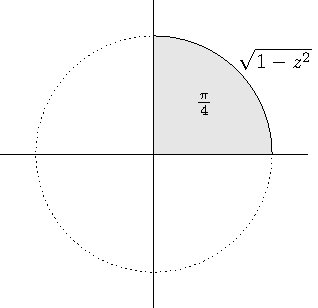
\includegraphics{images/circle-area}
  \caption{Berechnung der Fläche eines Kreises mit Radius $1$}%
  \label{fig:circle-area}
\end{figure}

\subsection*{Partialbruchzerlegung}
Die Partialbruchzerlegung ist eine Methode
zur Integration aller \emph{rationaler Funktionen}
auf $\mathbb{R}$,
das heisst, Funktionen der Form
$p/q$, wobei $p$ und $q$ Polynome sind.
Wir schreiben hier auch kurz $p, q \in \mathbb{R}[x]$.
Diese Notation wird spätestens in der Vorlesung
``Algebra'' gerechtfertigt.
Der Fall $q(x) = 1$ für alle $x$ entspricht einfach
der Integration eines Polynoms, was wir können.
Schwieriger ist es, Integrale der Form
\[
  \int_{a}^{b} \frac{1}{p(x)} \, dx
\]
zu berechnen.
Der Einfachheit halber beschränken wir uns auf diese Funktionen.

Sei
\(
  p(x) = x^n + a_1 x^{n-1} + a_2 x^{n-2} + \cdots
  + a_{n-1} x + a_n
\)
ein Polynom in $\mathbb{R}[x]$.
Wir betrachten den Spezialfall,
in dem $p$ genau $n$ paarweise verschiedene
Nullstellen $\alpha_1, \alpha_2, \dots, \alpha_n \in \mathbb{R}$ 
hat.
Daraus, dass das Polynom
\[
  x \mapsto p(x) - \prod_{x=1}^{n} (x - \alpha_k)
\]
höchstens Grad $n-1$ und genau $n$ Nullstellen
$\alpha_1, \dots, \alpha_n$ hat, folgt dass
\[
  p(x) = (x - \alpha_1) (x - \alpha_2) \cdots (x - \alpha_n)
\]
für alle $x \in \mathbb{R}$.

\begin{lemma}[Partialbruchzerlegung]\label{lem:partial-fractions}
  Sei $p \in \mathbb{R}[x]$ ein Polynom mit $n$ 
  paarweise verschiedenen Nullstellen
  $\alpha_1, \dots, \alpha_n$.
  Dann existieren $b_1, \dots, b_n \in \mathbb{R}$
  mit
  \[
    \frac{1}{p(x)} = \frac{b_1}{x - \alpha_1}
    + \cdots + \frac{b_n}{x - \alpha_n}.
  \]
\end{lemma}

\begin{application}
  Die Funktion
  \[
    x \mapsto \frac{b_k}{x - \alpha_k}
  \]
  hat Stammfunktion
  \[
    x \mapsto b_k \cdot \log (x - \alpha_k).
  \]
  Für ein Polynom $p \in \mathbb{R}[x]$ mit
  \[
    \frac{1}{p(x)} = \frac{b_1}{x - \alpha_1}
    + \cdots + \frac{b_n}{x - \alpha_n}
  \]
  folgt dann, dass
  \[
    \int_{a}^{b} \frac{1}{p(x)} \, dx
    = \sum_{k=1}^{n} \int_{a}^{b} \frac{b_k}{x - \alpha_k} \, dx
    = \sum_{k=1}^{n} b_k \cdot \log(b - \alpha_k)
    - \sum_{k=1}^{n} \log(a - \alpha_k),
  \]
  vorausgesetzt $\alpha_k \notin [a, b]$ für $k = 1, \dots, n$.
\end{application}

\begin{example}
  Sei $p(x) = (x - 1)(x - 2)$. Schreibe
  \[
    \frac{1}{p(x)} = \frac{b_1}{x - 1} + \frac{b_2}{x - 2}.
  \]
  Wir möchten $b_1$ und $b_2$ berechnen.
  Multiplizieren wir auf beiden Seiten mit $p(x)$,
  so erhalten wir
  \[
    1 = b_1 (x- 2) + b_2(x-1) = (b_1 + b_2) \cdot x
    + (-2b_1 - b_2).
  \]
  Es gilt also $b_1 + b_2 = 0$ und somit $b_2 = -b_1 = 1$.
\end{example}

\begin{proof}[Beweis von Lemma~\ref{lem:partial-fractions}]
  Um die Koeffizienten $b_k$ zu berechnen,
  machen wir den Ansatz
  \[
    \frac{1}{p(x)} = \sum_{k=1}^{n} \frac{b_k}{x - \alpha_k}.
  \]
  Schreibe
  \[
    p_k(x) = \frac{p(x)}{x - \alpha_k}.
  \]
  Bemerke, dass $p_k \in \mathbb{R}[x]$ ein Polynom
  von Grad $n-1$ ist, da $x - \alpha_k$ ein
  Faktor von $p$ ist.
  Multipliziere diesen Ansatz mit $p(x)$ und erhalte
  \[
    1 = \sum_{k=1}^{n} b_k \cdot p_k(x).
  \]
  Man bemerke, dass für $i \ne k$ gilt, dass
  $p_i(\alpha_k) = 0$, da $p_i$ den Faktor
  $x - \alpha_k$ enthält.
  Wir erhalten
  \[
    1 = \sum_{i=1}^{n} b_i \cdot p_i(\alpha_k) = b_k \cdot p_k(\alpha_k),
  \]
  also folgern wir
  \[
    b_k = \frac{1}{p_k(\alpha_k)}.
  \]
  Das macht Sinn, da $p_k(\alpha_k) \neq 0$.
 
  Wir behaupten nun, dass für diese $b_k$ tatsächlich
  \[
    \frac{1}{p(x)} = \sum_{k=1}^{n}  \frac{b_k}{x - \alpha_k}
  \]
  gilt.
  Bemerke dazu, dass die Abbildung
  \[
    x \mapsto 1 - \sum_{k=1}^{n} b_k p_k(x)
  \]
  ein Polynom vom Grad $n-1$ mit $n$ Nullstellen
  $\alpha_1, \dots, \alpha_n$ und somit die Nullfunktion ist.
  Wir erhalten, dass
  \[
    1 = \sum_{k=1}^{n} b_k p_k(x)
  \]
  für alle $x \in \mathbb{R}$.
  Division durch $p(x)$ liefert die Behauptung und somit
  das Lemma.
\end{proof}

\begin{issues}
  \leavevmode
  \begin{enumerate}[(i)]
    \item Das Polynom $p \in \mathbb{R}[x]$ könnte mehrfache
      Nullstellen haben, wie zum Beispiel
      das Polynom $p(x) = x^2 \cdot (x - 1)$.
    \item Das Polynom $p \in \mathbb{R}[x]$ hat vielleicht
      nicht nur reelle Nullstellen, wie zum Beispiel
      das Polynom $p(x) = x^2 + 1$.
  \end{enumerate}
\end{issues}

Das erste Problem lässt sich mit nicht allzu viel Aufwand lösen.
Schreibe
\[
  p(x) = {(x - \alpha_1)}^{k_1} \cdots
  {(x - \alpha_m)}^{k_m}.
\]
Dann liefert ein ähnlicher Beweis,
siehe Abschnitt 69 in~\cite{heuser},
eine Partialbruchzerlegung
\[
  \frac{1}{p(x)} = \sum_{i=1}^{m} \sum_{k=1}^{k_i} 
  \frac{c_{ik}}{{(x - \alpha_i)}^k}
\]
mit geeigneten Koeffizienten $c_{ik} \in \mathbb{R}$.
Auch dieses Resultat kann angewendet werden,
um Integrale
\[
  \int_{a}^{b} \frac{1}{p(x)} \, dx
  = \sum_{i=1}^{m} \sum_{k=1}^{k_i} \int_{a}^{b} 
  \frac{c_{ik}}{{(x - \alpha_i)}^k}\, dx
\]
zu berechnen.

\begin{example}
  Betrachte zum Beispiel das Polynom
    $p(x) = x^2 \cdot (x - 1)$.
  Mit dem Ansatz
  \[
    \frac{1}{p(x)} = \frac{a}{x^2} + \frac{b}{x}
    + \frac{c}{x-1}
  \]
  erhalten wir
  \begin{align*}
    1 & 
    = a(x - 1) + b x (x - 1) + cx^2\\
      &= (b + c) \cdot x^2 + (a - b) x - a.
  \end{align*}
  Wir folgern $b + c = a - b = 0$ und $a = -1$.
\end{example}
  
Für das zweite Problem verwenden wir den
\emph{Fundamentalsatz der Algebra},
der folgendes aussagt.

\begin{lemma}
  Sei $p \in \mathbb{C}[x]$ ein nicht-konstantes
  komplexes Polynom. Dann existiert $\alpha \in \mathbb{C}$ 
  mit $p( \alpha ) = 0$.
\end{lemma}

Für den Beweis, siehe Abschnitt 69 in~\cite{heuser}, oder
die Vorlesung ``Komplexe Analysis''.
Sei nun $p \in \mathbb{R}[x]$ und $\alpha = a + bi \in \mathbb{C}$ 
mit $p ( \alpha ) = 0$.
Dann gilt auch
$p(\overline \alpha) = 0$,
wobei $\overline \alpha = a - bi$
(hier brauchen wir, dass die Abbildung
$z \mapsto \overline z$ linear
und eingeschränkt auf $\mathbb{R}$ die Identität ist).
Es gilt nun
\[
  p(x) = (x - \alpha)(x - \overline \alpha) \widetilde{p}(x)
  = x^2 - 2ax + a^2 + b^2
\]

\begin{example}
  Sei $p(x) = x^3 + 2x^2 + x + 2$.
  Es gilt $p(i) = p(-i) = 0$.
  Wir folgern, dass $(x- i)(x + i) = x^2 + 1$ 
  das Polynom $p$ teilt. Tatsächlich gilt
  \[
    p(x) = (x^2 + 1)(x+2).
  \]
  In den Übungen ist $1/p(x)$ als
  \[
    \frac{1}{p(x)} = \frac{a}{x + 2}
    + \frac{bx + c}{x^2 + 1}
  \]
  zu schreiben. Unter Benutzung von
  \[
    \arctan'(x) = \frac{1}{x^2 + 1}
  \]
  lässt sich der Term $(bx + c)/(x^2 + 1)$ leicht integrieren.
\end{example}

\begin{remark}
  Sei $p \in \mathbb{R}[x]$ ein reelles Polynom mit
  einer Nullstelle $\alpha = a + ib \in \mathbb{C} \setminus \mathbb{R}$, das heisst, $b \neq 0$.
  Dann ist $p$ teilbar durch $(x - \alpha) (x - \overline \alpha)$,
  wobei $\overline \alpha = a - ib$.
  Es gilt
   \[
     (x - \alpha) ( x - \overline \alpha) = x^2 - 2ax + a^2 + b^2
     = {(x - a)}^2 + b^2.
  \]
  Nach einer linearen Substitution $x \mapsto x - a$
  erhalten wir den Faktor $x^2 + b^2$.
  Um $1/p(x)$ zu integrieren, müssen wir wir insbesondere
  $1/(x^2 + b^2)$ integrieren können.
  Dazu betrachte die Tangensfunktion
  \begin{align*}
    \tan \colon (-\pi/2, \pi/2) & \to \mathbb{R} \\
    x & \mapsto \frac{\sin(x)}{\cos(x)}.
  \end{align*}
  Wir berechnen
  \begin{align*}
    \tan'(x)
    &=\frac{\sin'(x)}{\cos(x)} + \sin(x) \cdot
    \left( - \frac{\cos'(x)}{\cos^2(x)} \right)\\
    &= 1 + \tan^2(x) \\
    &\geq 1
  \end{align*}
  für alle $x \in (-\pi/2, \pi/2)$.
  Insbesondere hat $\tan$ eine differenzierbare Umkehrfunktion
  \[
    \arctan \colon \mathbb{R} \to (- \pi/2, \pi/2).
  \]
  Es gilt
  \begin{align*}
    \arctan'(x)
    & = \frac{1}{1 + {\tan(\arctan(x))}^2}\\
    & = \frac{1}{1 + x^2}
  \end{align*}
  Für $b > 0$ gilt nun
  \[
    \left( \frac{1}{b} \cdot \arctan \left( \frac{x}{b} \right) \right)'
    = \frac{1}{b} \cdot \frac{1}{1 + {(x/b)}^2} \cdot \frac{1}{b}
    = \frac{1}{b^2 + x^2}.
  \]
  
  
  
  
  
  
\end{remark}



\end{document}
